\section{Real-time performance}
\label{sec:prediction_performance}

The real-time performance of the our application has always been the main bottleneck, in that it needs to run in real-time and provide arrival time predictions as soon as possible after the data is received. During the simulation run to obtain the results from \cref{sec:prediction_model_comparison}, we also recorded the timings of individual parts of the program, of which overall averages are displayed in \cref{tab:prediction_timing}. In it, we have two timers: wall clock and CPU clock. Wall clock is the real-world time passed, while the CPU clock is the time spent on the processor.  We ran the simulation using four~cores, which affects the vehicle update (V) and \gls{eta} prediction (P) steps, as these are run in parallel. The other steps are not parallelised, so the wall and CPU timings are approximately similar, with the exception of the Load data (L) step, which involves calling the \gls{gtfs} \gls{api} and waiting for the data to download.


On average, the program takes less than five~seconds, which is well below our original target of 30~seconds. The most intensive component is updating of vehicle states, which involves updating 10,000 particles for each operating vehicle. This is followed by the \gls{eta} prediction step, which involves far fewer particles (we used 200 per trip), but each particle is required to estimate more per iteration [better wording]. However, the main advantage is that, in the vehicle update step, we perform a full weighted resample of the particles, which involves a full copy of all $\Np$ particles, plus sorting (if applicable). In the \gls{eta} step, we are able to use a single pointer to iterate over sampled particles, which completely avoids any copying.


\begin{knitrout}\small
\definecolor{shadecolor}{rgb}{0.969, 0.969, 0.969}\color{fgcolor}\begin{table}

\caption{\label{tab:prediction_timing}Time taken, in milliseconds, during various parts of the program, running on a single core.}
\centering
\fontsize{8}{10}\selectfont
\begin{tabular}[t]{lrlrl}
\toprule
 & Wall clock & (SE) & CPU time & (SE)\\
\midrule
(L) Load data & 29 & (0.21) & 17 & (0.19)\\
(U) Update vehicle information & 3.37 & (0.039) & 3.29 & (0.034)\\
(V) Vehicle state update & 3190 & (33) & 10300 & (97)\\
(N) Network state update & 0.458 & (0.012) & 1.35 & (0.026)\\
(P) Predict ETAs & 1310 & (27) & 3170 & (37)\\
\addlinespace
(W) Write ETAs to protobuf feed & 162 & (0.57) & 189 & (0.53)\\
\midrule
(T) Total iteration time & 4690 & (51) & 13700 & (130)\\
\bottomrule
\end{tabular}
\end{table}


\end{knitrout}


However, there is a high level of variability in the number of buses operating at any given time (figure X), so in \cref{fig:prediction_timing_time} we have displayed the timings for each individual iteration over the course of the day. We again see the peak hour effect, where there are upwards of 1000~vehicles operating. This pushes the total iteration time to a between 10 and 15~seconds, which is still well within our target of 30~seconds. We could slightly increase the number of particles, although it is worth remembering that the \emph{resampling} step of the particle filter has a computational complexity of $\mathcal{O}(N\log N)$, so for example we cannot double the number of particles and expect to remain under the 30~second target.
\textcolor{red}{Note to self: re-run simulations overnight, when you're not also using the CPU cores for other tasks, which should remove the oddity between about 9am and 2pm.}


\begin{knitrout}\small
\definecolor{shadecolor}{rgb}{0.969, 0.969, 0.969}\color{fgcolor}\begin{figure}

{\centering 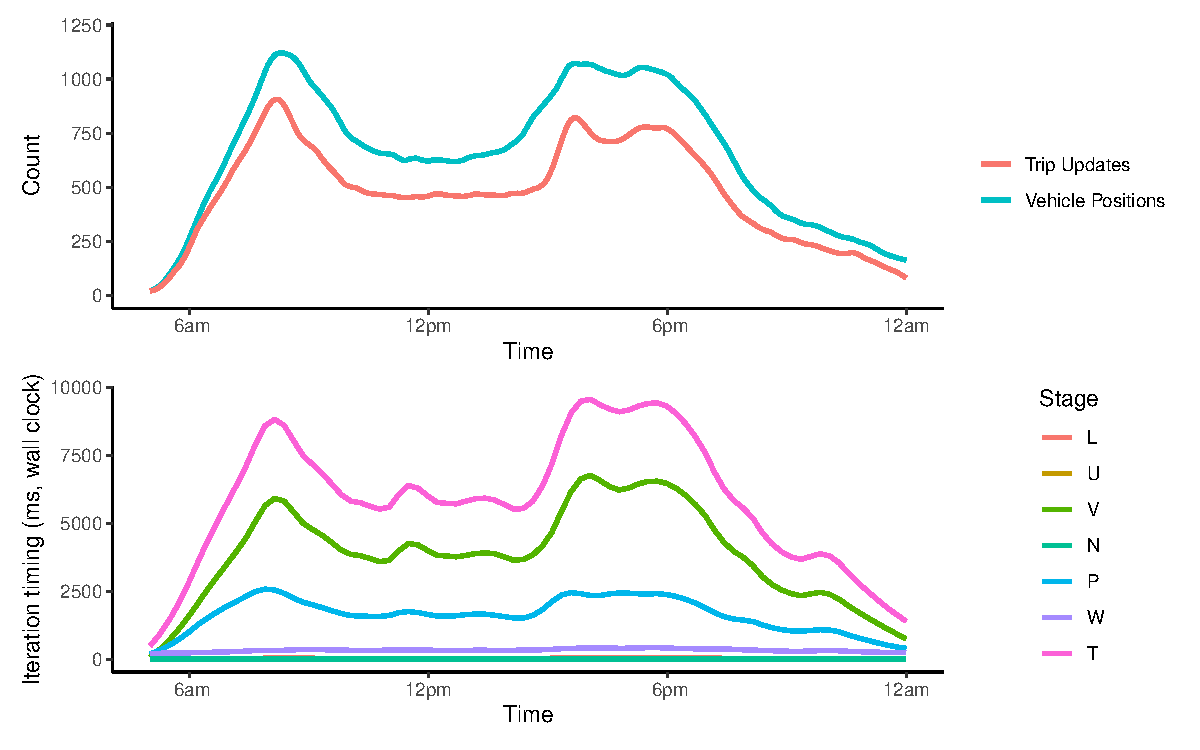
\includegraphics[width=.8\textwidth]{figure/prediction_timing_time-1} 

}

\caption[Timing results over time for various stages of the program]{Timing results over time for various stages of the program: (L) Load data, (O) Update vehicles information, (V) Vehicle state update, (N) Network state update, (P) Predict ETAs, (W) Write ETAs to protobuf feed, (T) Total iteration time.}\label{fig:prediction_timing_time}
\end{figure}


\end{knitrout}
